%Este trabalho está licenciado sob a Licença Creative Commons Atribuição-CompartilhaIgual 3.0 Não Adaptada. Para ver uma cópia desta licença, visite https://creativecommons.org/licenses/by-sa/3.0/ ou envie uma carta para Creative Commons, PO Box 1866, Mountain View, CA 94042, USA.
% !TEX root = ../main.tex
\chapter{Superfícies}
Neste capítulo, estudaremos funções vetoriais do tipo $\vec{f}(u,v)$, ou seja, uma função que associa um ponto do plano real a vetores no espaço.
\section{Funções vetoriais de duas variáveis reais - superfícies}
Uma função vetorial de duas variáveis é uma função da forma $$\vec{r}:D_1\times D_2 \to \mathbb{R}^3,$$ onde $D_1\times D_2\subseteq \mathbb{R}^2$ é o domínio de definição de $\vec{r}$ e $(u,v)\in D_1\times D_2$ são os parâmetros ou as coordenadas de superfície. Em coordenadas cartesianas, uma função vetorial assume a seguinte forma:
$$\vec{r}(u,v)=x(u,v)\vec{i}+y(u,v)\vec{j}+z(u,v)\vec{k}$$
\begin{ex}\label{exfv_1} São exemplos de funções vetoriais
\begin{itemize}
\item [a)] $\vec{f}(u,v)=\sin(u)\vec{i}+\cos(v)\vec{j}+uv\vec{k}$
\item [b)] $\vec{g}(u,v)=\sin(u)\cos(v) \vec{i}+\cosh(u)\sinh(v)\vec{j}+u\vec{k}$
\end{itemize}
\end{ex}

As derivadas parciais, limites e integrais são definidas termo a termo, semelhante ao estudo de curvas do capítulo anterior. 
\begin{ex}
 Dada a função vetorial $\vec{r}(u,v)=u\vec{i}+\sin(v)\vec{j}+e^{uv}\vec{k}$, temos $\vec{r}_u=\vec{i}+ve^{uv}\vec{k}$ e $\vec{r}_v=\cos(v)\vec{j}+ue^{uv}\vec{k}$.
\end{ex}


Uma superfície\index{superfície} no espaço pode ser representada pelo conjunto de pontos de uma função vetorial $\vec{r}(u,v)$ não constante em todo o seu domínio. A seguinte interpretação ajuda entender essa função: se fixamos $v$ e temos que $\vec{r}(u,v)$ descreve uma curva e $\vec{r}_u(u,v)$ é um vetor tangente a essa curva. Da mesma forma, se fixamos $u$ temos que $\vec{r}(u,v)$ descreve uma curva e $\vec{r}_v(u,v)$ é um vetor tangente a essa curva. Se essas curvas não forem paralelas, temos um sistema de coordenadas curvilíneo para escrever todos os pontos da superfície. Pense no globo terrestre, o medidiano de Greenwich e a linha do Equador: o globo como uma superfície, Greenwich e Equador como duas curvas e longitude e latitude como um sistema de coordenadas curvilíneo, veja Figura~\ref{cap_superficies_esfera} Observe que esse sistema curvilíneo fica bem definido quando $\vec{r}_u$ e $\vec{r}_v$ não são paralelos nos pontos do domínio. Chamamos de superfície regular aquela que satisfaz
$$
\vec{r}_u\times \vec{r}_v\neq \vec{0}.
$$
\begin{ex}A função vetorial
$$
\vec{r}=a\sin(u)\cos(v)\vec{i}+a\sin(u)\sin(v)\vec{j}+a\cos(u)\vec{k},~~ a>0, ~ 0\leq u< \pi, ~ 0\leq v< 2\pi
$$
descreve uma esfera centrada na origem e raio $a$. De fato, colocando $$x=a\sin(u)\cos(v),\qquad y=a\sin(u)\sin(v)\qquad\text{e}\qquad z=a\cos(u),$$
temos que
$$
x^2+y^2+z^2=a^2.
$$
Além disso, se $(x,y,z)$ é um ponto qualquer nesta esfera, então existem $u$ e $v$ na parametrização. Para tal, basta escolher $u=\cos^{-1}\left(\frac{z}{a}\right)$ e escolher $v\in[0,2\pi)$ tal que:
$$\cos(v)=\frac{x}{a\sin(u)} \quad \hbox{e} \quad \sin(v)=\frac{y}{a\sin(u)},~~u\neq 0 ~~ \hbox{e} ~~u\neq \pi.$$

 \begin{figure}%{r}{8cm}
\centering
 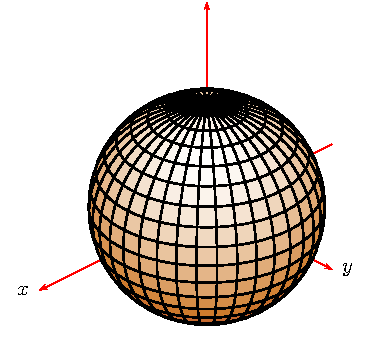
\includegraphics{cap_superficies/figs/figura_1}\label{cap_superficies_esfera}
\caption{Uma esfera centrada na origem com meridianos e paralelos traçados.}
\end{figure}
\end{ex}

\begin{ex}A função vetorial
 $$
 \vec{r}=\cosh(u)\cos( v)\vec{i}+ \cosh(u)\sin(v)\vec{j}+\sinh(u)\vec{k},\ 0\leq v\leq 2\pi,\ u\in\mathcal{R}
 $$
 descreve um hiperbolóide de uma folha. De fato, para cada par $(u,v)$ no domínio, a parametrização
 $$
 x(u,v)=\cosh(u)\cos(v),\qquad y(u,v)=\cosh(u)\sin(v)\quad\text{e}\quad z(u,v)=\sinh(u)
 $$
 nos leva na equação canônica de um hiperbolóide de uma folha:
 \begin{eqnarray*}
 x^2+y^2-z^2&=&\cosh^2(u)\cos^2(v)+\cosh^2(u)\sin^2(v)-\sinh^2(u)  \\
 &=&\cosh^2(u)(\cos^2(v)+\sin^2(v))-\sinh^2(u)  \\
 &=&\cosh^2(u)-\sinh^2(u)  \\
 &=&1.
 \end{eqnarray*}
Recriprocamente, se $(x,y,z)$ é um ponto sobre o hiperbolóide, definimos $u=\sin^{-1}(z)$ e escolhemos $v\in[0,2\pi)$ tal que:
$$\cos(v)=\frac{x}{\cosh(u)} \quad \hbox{e} \quad \sin(v)=\frac{y}{\cosh(u)}.$$
 \end{ex}
 
 \subsection*{Exercícios}
 \begin{exer}Mostre que a função vetorial
  $$
  \vec{r}(u,v)=(u+v)\vec{i}+(u-v)\vec{j}+(3u-2v+1)\vec{k}, \qquad 0\leq u,v\leq \infty,
  $$
  descreve um plano.
 \end{exer}

 \begin{exer}Mostre que a função vetorial
  $$
  \vec{r}(u,v)=3\cos(u)\vec{i}+3\sin(u)\vec{j} +v\vec{k}, \qquad 0\leq u\leq 2\pi,\quad 0\leq v\leq 2
  $$
  descreve um cilíndro.
 \end{exer}
 
 
\section{Vetor unitário normal e orientação}\index{vetor normal à uma superfície}
Para os fins de teoria de integraçao sobre superfícies, que discutiremos mais adiante, é fundamental definir o vetor unitário normal. Dado uma superfície e um ponto nela, dizemos que um vetor é normal à superfície se ele é perpendicular no ponto a cada curva contida na superfícies. Em especial, um vetor normal à superfícies no ponto $x_0=x(u_0,v_0)$, $y_0=y(u_0,v_0)$ e $z_0=z(u_0,v_0)$, deve ser perpendicular às curvas $\vec{r}(u_0,v)$ e $\vec{r}(u,v_0)$, isto é, as curvas geradas quando se fixa um dos parâmetros $u_0$ ou $v_0$, respectivamente. Assim, podemos concluir que cada vetor normal está da mesma direção do produto vetorial $\vec{r}_u\times\vec{r}_v$. Finalmente, o vetor normal unitário deve ter norma unitária, portanto, deve ser da forma:
\begin{equation}\label{cap_superficies_normal_unitario}
 \vec{n} = \pm \frac{\vec{r}_u\times\vec{r}_v}{\|\vec{r}_u\times\vec{r}_v\|}.
\end{equation}
Observe que se a superfície for regular, então $\vec{r}_u\times\vec{r}_v\neq \vec{0}$, o que indica que a expressão \eqref{cap_superficies_normal_unitario} está bem definida. Aqui, o sinal indica para qual lado o vetor normal aponta e define a orientação da superfície. 

\begin{ex}Vamos calcular o vetor normal à esfera
$$
\vec{r}=a\sin(u)\cos(v)\vec{i}+a\sin(u)\sin(v)\vec{j}+a\cos(u)\vec{k},~~ a>0, ~ 0\leq u< \pi, ~ 0\leq v< 2\pi
$$
Calculamos as derivadas
\begin{eqnarray*}
\vec{r}_u&=&a\cos(u)\cos(v)\vec{i}+a\cos(u)\sin(v)\vec{j}-a\sin(u)\vec{k},\\
\vec{r}_v&=&-a\sin(u)\sin(v)\vec{i}+a\sin(u)\cos(v)\vec{j},
\end{eqnarray*}
o produto vetorial
\begin{eqnarray*}
\vec{r}_u\times \vec{r}_v&=&\left[\begin{array}{ccc}
                                \vec{i}&\vec{j}&\vec{k}\\
                                a\cos(u)\cos(v)&a\cos(u)\sin(v)&-a\sin(u)\\
                                -a\sin(u)\sin(v)&a\sin(u)\cos(v)&0
                                \end{array}
\right]\\
&=&a^2\sin^2(u)\cos(v)\vec{i}+a^2\sin^2(u)\sin(v)\vec{j}\\&+&(a^2\sin(u)\cos(u)\cos^2(v)+a^2\sin(u)\cos(u)\sin^2(v))\vec{k}\\
&=&a^2\sin^2(u)\cos(v)\vec{i}+a^2\sin^2(u)\sin(v)\vec{j}+a^2\sin(u)\cos(u)\vec{k}
\end{eqnarray*}
e a norma do produto vetorial
\begin{eqnarray*}
\|\vec{r}_u\times \vec{r}_v\|&=&a^2\sqrt{\sin^4(u)\cos^2(v)+\sin^4(u)\sin^2(v)+\sin^2(u)\cos^2(u)}\\
&=&a^2\sqrt{\sin^4(u)+\sin^2(u)\cos^2(u)}\\
&=&a^2\sqrt{\sin^2(u)}\\
&=&a^2\sin(u),
\end{eqnarray*}
visto que $0\leq u< \pi$. Assim,
\begin{eqnarray*}
\vec{n}&=&\pm \frac{\vec{r}_u\times \vec{r}_v}{\|\vec{r}_u\times \vec{r}_v\|}\\
&=&\pm\frac{a^2\sin^2(u)\cos(v)\vec{i}+a^2\sin^2(u)\sin(v)\vec{j}+a^2\sin(u)\cos(u)\vec{k}}{a^2\sin(u)}\\
&=&\pm\left(\sin(u)\cos(v)\vec{i}+\sin(u)\sin(v)\vec{j}+\cos(u)\vec{k}\right).
\end{eqnarray*}
Observe que em $u=v=0$, temos $\vec{r}=a\vec{k}$ e $\vec{n}=\pm\vec{k}$. Portanto, o sinal positivo orienta a superfície para fora e o sinal negativo orienta a superfície para dentro.
\end{ex}

\subsection*{Exercícios resolvidos}

\begin{exeresol} 
Calcule o vetor normal unitário à superfície cônica $z=1-\sqrt{x^2+y^2}$ no ponto $(1,0,0)$, sabendo que a orientação positiva tem componente $\vec{k}$ negativa. 
\end{exeresol}
\begin{resol}
 Considere a parametrização para o cone $\vec{r}(x,y)=x\vec{i}+y\vec{j}+(1-\sqrt{x^2+y^2})\vec{k}$. Calculamos
\begin{eqnarray*}
\vec{r}_x&=&\vec{i}-\frac{x}{\sqrt{x^2+y^2}}\vec{k},\\
\vec{r}_y&=&\vec{j}-\frac{y}{\sqrt{x^2+y^2}}\vec{k}.
\end{eqnarray*}
No ponto $(1,0)$, temos:
\begin{eqnarray*}
\vec{r}_x&=&\vec{i}-\vec{k},\\
\vec{r}_y&=&\vec{j},
\end{eqnarray*}
O produto vetorial é dado por
\begin{eqnarray*}
\vec{r}_x\times \vec{r}_y&=&\vec{i}+\vec{k}
\end{eqnarray*}
e a norma do produto vetorial
\begin{eqnarray*}
\|\vec{r}_x\times \vec{r}_y\|&=&\sqrt{2}.
\end{eqnarray*}
Assim,
\begin{eqnarray*}
\vec{n}&=&\pm \frac{\vec{r}_x\times \vec{r}_y}{\|\vec{r}_x\times \vec{r}_y\|}\\
&=&\pm\frac{\sqrt{2}}{2}\left(\vec{i}+\vec{k}\right).
\end{eqnarray*}
Como a orientação positiva da superfície tem componente $\vec{k}$ negativa, o vetor normal é
\begin{eqnarray*}
\vec{n}&=&-\frac{\sqrt{2}}{2}\left(\vec{i}+\vec{k}\right).
\end{eqnarray*}
\end{resol}



\subsection*{Exercícios}
\begin{exer}
Calcule o vetor normal unitário ao parabolóide $z=x^2+y^2$ no ponto $(1,1,2)$, sabendo que a orientação positiva tem componente $\vec{k}$ positiva.  
\end{exer}
   



\section{Caso particular em que a superfície é o gráfico de uma função}
O caso particular da superfície representada por uma função $z=f(x,y)$, podemos assumir uma parametrização natural $\vec{r}=u\vec{i}+v\vec{j}+f(u,v)\vec{k}$. Analogamente para os casos $y=f(x,z)$ ou $x=f(y,z)$, podemos assumir, respectivamente, as parametrizações $\vec{r}=u\vec{i}+f(u,v)\vec{j}+v\vec{k}$ ou $\vec{r}=f(u,v)\vec{i}+v\vec{j}+u\vec{k}$. Para o caso $z=f(x,y)$ (analogamente para os demais), a condição $\vec{r}_u\times \vec{r}_v\neq \vec{0}$ assume a forma
\begin{eqnarray*}
 \vec{r}_u\times \vec{r}_v&=&\left|\begin{array}{ccc}\vec{i}&\vec{j}&\vec{k}\\ 1&0&f_u(u,v)\\0&1&f_v(u,v)\end{array} \right|\\&=&-f_u\vec{i}-f_v\vec{j}+\vec{k}\neq \vec{0}.
\end{eqnarray*}
Isso implica que $ \vec{r}_u\times \vec{r}_v \neq 0$, ou seja, a superfície \'{e} regular. Voltaremos a discutir esse assunto nos próximos capítulos, quando o vetor gradiente estiver definido.

\begin{ex}Os planos são definidos por equações da forma
$$
ax+by+cz+d=0,
$$
onde pelo menos umas das constante $a$, $b$ ou $c$ não é zero. Supondo $c\neq0$, basta escrever $z=f(x,y)=\frac{-ax-by-d}{c}$ e definimos o plano como o gráfico da função $f$.
\end{ex}

\begin{ex}
A figura \ref{quadricas} apresenta uma lista das principais quádricas\index{quádricas} estudadas na disciplina de Cálculo Diferencial e Integral com funções de várias variáveis. As equações são as seguintes:
\begin{itemize}
\item[a)] Cone elíptico: $\displaystyle z^2=\frac{x^2}{a^2}+\frac{y^2}{b^2}$.
\item[b)] Elipsóide: $\displaystyle \frac{x^2}{a^2}+\frac{y^2}{b^2}+\frac{z^2}{c^2}=1$
\item[c)] Parabolóide Elíptico: $\displaystyle z=\frac{x^2}{a^2}+\frac{y^2}{b^2}$
\item[d)] Parabolóide Hiperbólico: $\displaystyle z=\frac{x^2}{a^2}-\frac{y^2}{b^2}$
\item[e)] Hiperbolóide de uma folha: $\displaystyle \frac{x^2}{a^2}+\frac{y^2}{b^2}-\frac{z^2}{c^2}=1$
\item[f)] Hiperbolóide de duas folhas:  $\displaystyle -\frac{x^2}{a^2}-\frac{y^2}{b^2}+\frac{z^2}{c^2}=1$
\end{itemize}
\begin{figure}[htp]
\begin{minipage}{5cm}
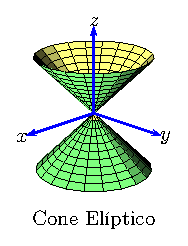
\includegraphics{cap_superficies/figs/figura_2}
\end{minipage}\begin{minipage}{5cm}
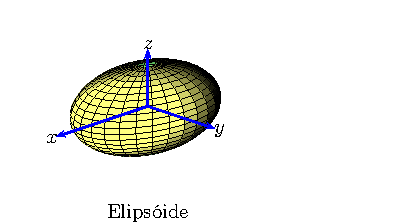
\includegraphics{cap_superficies/figs/figura_3}
\end{minipage}\begin{minipage}{5cm}
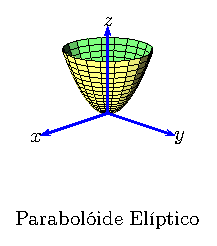
\includegraphics{cap_superficies/figs/figura_4}
\end{minipage}

\begin{minipage}{5cm}
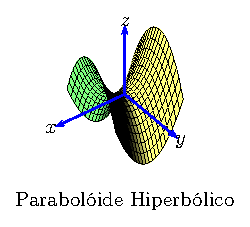
\includegraphics{cap_superficies/figs/figura_5}
\end{minipage}\begin{minipage}{5cm}
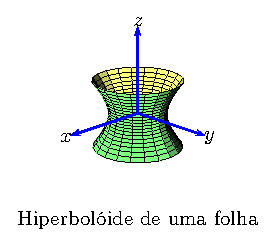
\includegraphics{cap_superficies/figs/figura_6}
\end{minipage}\begin{minipage}{5cm}
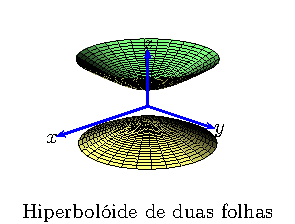
\includegraphics{cap_superficies/figs/figura_7}
\end{minipage}
\caption{\label{quadricas}Quádricas}
\end{figure}

Algumas das superfícies quádricas são gráficos de funções, como é o caso dos parabolóides e outras não são, como é o caso cone elíptico. Mesmo assim, podemos definir a quádrica como a união do gráfico de duas funções. Por exemplo, o cone elíptico pode ser escrito como a união dos gráficos das funções $z=\sqrt{\frac{x^2}{a^2}+\frac{y^2}{b^2}}$ e $z=-\sqrt{\frac{x^2}{a^2}+\frac{y^2}{b^2}}$.
\end{ex}

\begin{ex}A superfície cilíndrica $x^2+y^2=9$, $0\leq z\leq 2$, pode ser escrita como a união dos gráficos das funções $x=\sqrt{9-y^2}$, $0\leq z\leq 2$ e $x=-\sqrt{9-y^2}$, $0\leq z\leq 2$.
\end{ex}

\subsection*{Exercícios}
\begin{exer}Esboce o gráfico da superfície $z=1-x^2-y^2$, $z\geq0$.
\end{exer}
\begin{exer}Esboce o gráfico da superfície $z=1-\sqrt{x^2+y^2}$, $z\geq0$.
\end{exer}
\begin{exer}Esboce o gráfico da superfície $y^2+z^2=4$, $0\leq x\geq 3$.
\end{exer}
\begin{exer}Esboce o gráfico da superfície $x+y+z=1$, no primeiro octante.
\end{exer}

